\chapter{Introduction}\label{ch:intr}
The phenomena of heavy-tailedness is widely observed in many
disciplines of science, for example, phase transition of matter and
black body radiation as studied in physics, neuronal avalanches in
biology, claim sizes of insurance mathematics and stock returns in
finance. The last application is indeed the focus of this thesis. To
discuss the phenomena in precise terms, we introduce the concept of
regular variation.

\section{Regular Variation}
The concept of regular variation is defined by the following scaling
property: if a function $f(\cdot)$ satisfies
\[
\lim_{x \to \infty} {f(c x) \over f(x)} = c^\alpha
\quad
\forall c > 0
\]
then we say $f(x)$ is regularly varying with index $\alpha$.
% Distribution functions, say $F(\cdot)$, whose survival function
% $\bar F(x) = 1 - F(x)$ satisfies the above scaling property, are
% observed in a variety of phenomena, 
When expanded to multiple dimensions, the scaling property of regular
variation is better described in terms of vague convergence to a
spectral measure $\mu_\alpha$: if a random vector $V$ satisfies
\[
{
  \P(V/|V| \in \cdot, |V| > c x)
  \over
  \P(|V| > x)
},
\overset{v}{\to} c^{-\alpha} \mu_\alpha(\cdot)
\quad
x \to \infty, \forall c > 0
\]
then we say the $V$ is regularly varying with index $\alpha$. Here
$\mu_\alpha(\cdot)$ is a probability measure on the unit sphere
\cite{buraczewski:damek:mikosch:2016}. Clearly, if $V$
is regularly varying with index $\alpha$, then each component
of it and each linear combination of its components are regularly
varying with the same index $\alpha$. This follows from Feller
\cite{feller}, p. 278. Cf. also Jessen and Mikosch
\cite{JessenMikosch2006}, lemma 3.1, and Embrechts et. al.
\cite{embrechts:klueppelberg:mikosch:1997}, lemma 1.3.1.

Clearly, estimating the tail index $\alpha$ is particularly important
for understanding the behaviour of a heavy-tailed series. A standard
method proposed for this purpose is due to Hill \cite{hill1975simple}:
\[
\hat \alpha_H = \left[
  {1 \over k} \sum_{i=1}^k \log \left(
  X_{(i)} \over X_{(k+1)}
  \right)
  \right]^{-1}
\]
where $X_1, X_2, \dots$ is the series whose tail index is the subject
of estimation, and $X_{(i)}$ is the $i$-th upper order statistics of
this series. Several authors have contributed to showing the
weak consistency of the estimator $\hat \alpha_H$,
i.e. if $k \to \infty, k/n \to 0$ as $n \to \infty$, then
$\hat \alpha_H \overset{P}{\to} \alpha$.

Mason \cite{mason:1982} first proved that the estimator
was consistent when $X_1, X_2, \dots$ were iid; later Rootz\'en,
Leadbetter and de Haan \cite{rootzen:leadbetter:dehaan1992} and Hsing
\cite{hsing:1991} proved its consistency when $X_1, X_2, \dots$ were
weakly dependent; and Resnick and St{\u a}ric{\u a}
\cite{resnick:starica:1995, resnick:starica:1997} proved its
consistency when $X_t$ was a linear process.

Figure \ref{fig:thjyuj} shows the Hill estimates of the tail indices
of daily stock return series from 3 sectors of the
{\em Standard \& Poor 500} index \footnote{An American stock index
  comprising 500 or so companies.}. The 2.5\% and 97.5\% quantiles of
the asymptotic normal distribution of the estimates are also
given. One can see the confidence bands are fairly large compared with
the estimated values. This certainly raises the question of how
similar they really are and if/how their variations can be explained by
economical arguments. We explore this topic in chapter
\ref{ch:TailParameters}.

\begin{figure}[htb!]
  \begin{minipage}{1.0\linewidth}
    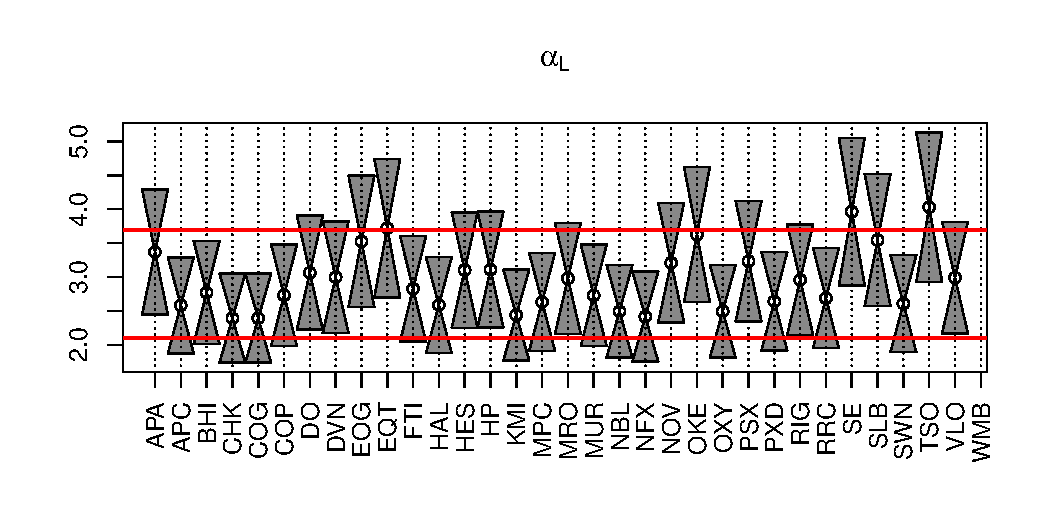
\includegraphics[width=\textwidth, trim={0, 0.8cm, 0, 2cm}, clip]
    {Energy_lower.pdf}
  \end{minipage}
  \begin{minipage}{1.0\linewidth}
    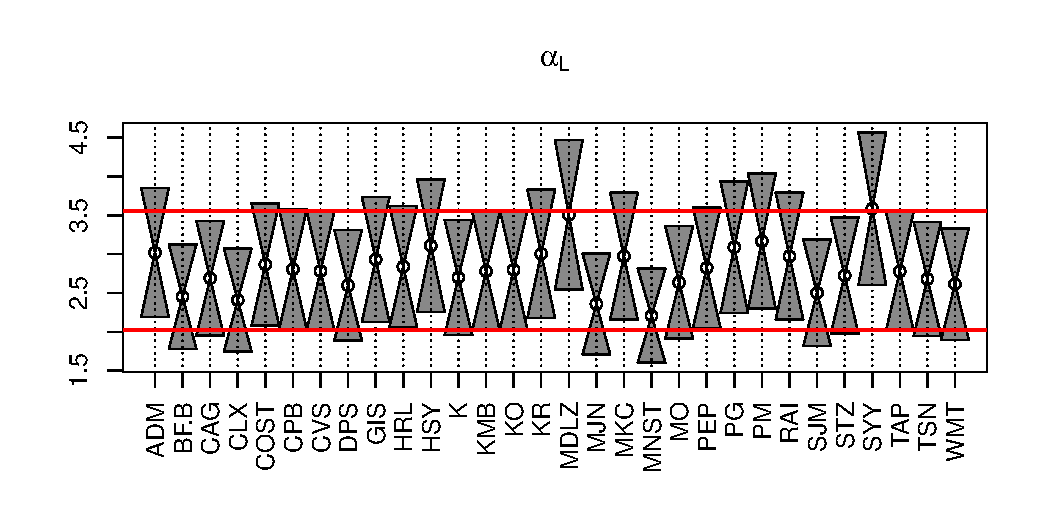
\includegraphics[width=\textwidth, trim={0, 0.8cm, 0, 2cm}, clip]
    {Consumer_Staples_lower.pdf}
  \end{minipage}
  \begin{minipage}{1.0\linewidth}
    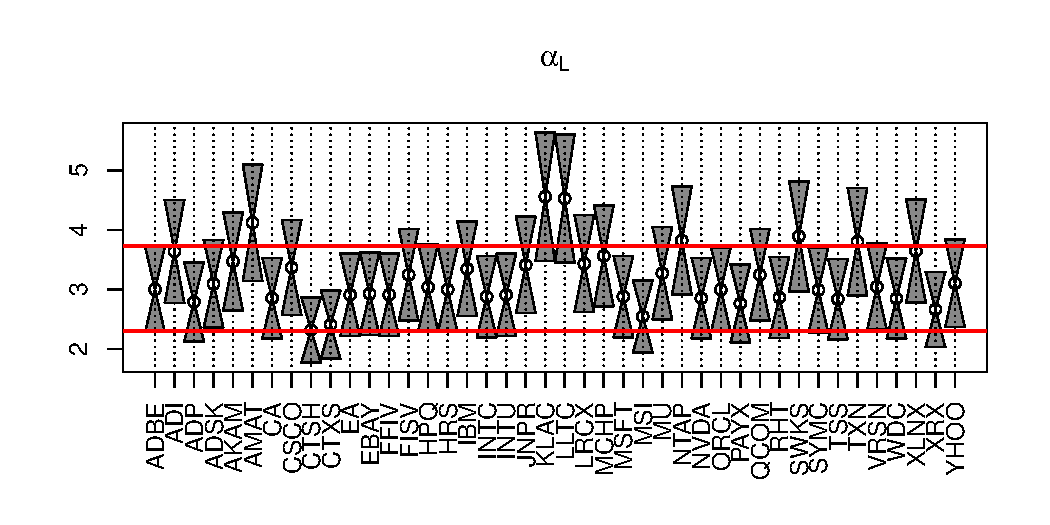
\includegraphics[width=\textwidth, trim={0, 0.8cm, 0, 2cm}, clip]
    {Information_Technology_lower.pdf}
  \end{minipage}
  \caption{\small Hill estimates $\hat \alpha_{50}$ of the lower
    tail-indices $\alpha$ of daily return series in sectors of the S\&P 500
    index. The data span from 1 January 2010 to 31 December 2014 and
    comprise $n=1304$ observations.
    The graphs from top to bottom correspond to the ``Energy'',
    ``Consumer Staples'' and ``Information Technology'' sectors.
    Each circle corresponds to a Hill estimate $\hat\alpha_{50}$; the gray
    triangles above and below it mark the 97.5\% and 2.5\% quantiles
    of its approximate normal distribution; see \eqref{eq:2} and the
    discussion following it for an interpretation.
    The lower and upper red lines mark the medians of the 2.5\% 
    and 97.5\% quantiles, respectively, evaluated from all stocks in
    the sector.
    The data are taken from {\it Yahoo Finance}; the labels on
    the horizontal axes are Yahoo symbols of the stocks. 
  }\label{fig:thjyuj}
\end{figure}

Random variables with regularly varying tails have some very nice
features: if $X_1$ and $X_2$ are both regularly varying with indices
$\alpha_1$ and $\alpha_2$, respectively, then $a_1 X_1 + a_2 X_2$ is
regularly varying with index $\min\{\alpha_1, \alpha_2\}$. Moreover
if $X_1, X_2$ are iid,
$\P(a_1 X_1 + a_2 X_2 > u) \sim \P(a_1 X_1 > u) + \P(a_2 X_2 > u)$.

Now consider $N$ return series $X_{i,t}$, $i=1,2,\dots, p$. Suppose
each of these series is a linear combination of $K$ factors $Y_{i,t}$,
$i=1,2,\dots,K$, the $i$-th of which is regularly varying with index
$\alpha_i$. Then by the summation property, each and every $X_i$ is
regularly varying with index $\min_{1 \leq i \leq K} \alpha_i$.
Since in practice a factor $Y_{i,t}$ is found as a linear combination
of $X_{i,t}$, the observed time series, following an eigenvector of
the sample covariance matrix of $X_{i,t}$, it is important to
understand the eigensystem of this matrix. This topic indeed
constitutes chapters \ref{ch:bernoulli} and \ref{ch:extremes} of this
thesis.

When a product of random variables, say $X_1 X_2$, involves a random
variable with regularly varying tails, a useful result is that of
Breiman: assume $X_1$ is regularly varying with index $\alpha$ and
there exists $\epsilon > 0$ such that
$\E |X_2|^{\alpha + \epsilon} < \infty$.
Then $\P(X_1 X_2 > x) \sim \E|X_2|^{\alpha} \P(X_1 > x)$.
More generally, if $X_1, X_2$ are regularly varying with the same tail
index $\alpha$ or if $\P(X_2 > x) = o(\P(X_1 > x))$, then $X_1 X_2$ is
regularly varying with index $\alpha$.

For an extensive summary of the regular variation properties of
functions of regularly varying random variables, see Mikosch and
Jessen \cite{JessenMikosch2006}.

% When considered as the multiplicative inverse of the parameter of the
% {\em Generalized Extreme Value} distribution, there are other methods
% in the literature for estimating the tail index, e.g. Pickand's 
% estimator \cite{pickands1975statistical} $\hat \alpha_P$ and the
% Deckers-Einmahl-de Haan estimator $\hat \alpha_{\text{DEH}}$
% \begin{eqnarray*}
% {1 \over \hat \alpha_P}
% &=&
% {1 \over \log 2}
% \log {
%   X_{(k)} - X_{(2k)}
%   \over
% X_{(2k)} - X_{(4k)}  
% } \\
% {1 \over \hat \alpha_{\text{DEH}}}
% &=&
% 1 + {1 \over \alpha_H} + {1 \over 2} \left(
%   {H \over \alpha_H^2} - 1
% \right)^{-1}
% \end{eqnarray*}
% where it is similarly assumed $k \to \infty$ and $k/n \to 0$ as $n \to
% \infty$. The Deckers-Einmahl-de Haan estimator makes use of Hill's
% estimator $\hat \alpha_H$ and computes
% \[
% H = \left[
%   {1 \over k} \sum_{i=1}^k \log \left(
%     { X_{(i)} \over X_{(k+1)} }
%   \right)^2
% \right]^{-1}
% \]
% Apparently $1/H$ can be interpreted as the 2nd empirical moment of
% $\log(X_{(i)}/X_{(k+1)})$ for $i \leq k$.
% A major drawback of Pickand's and Deckers-Einmahl-de Haan's estimators
% is that, when applied to estimating the tail index, they discard the
% information that the tail index is always positive, hence resulting in
% a larger confidence band compared with that obtained for Hill's
% estimator. Therefore we stick to Hill's estimator in the empirical
% work included in this thesis.

\section{Stochastic Recurrence Equation}
One of the most important dynamical mechanisms that lead to regularly
varying r.v. is stochastic recursion of the following form:
\begin{equation}
  \label{eq:rhjyu}
  X_t = A_t X_{t-1} + B_t
\end{equation}
where $X_t$ is a $d$-dimensional random vector, $A_t$ is a $d\times d$
random matrix and $B_t$ is a $d$-dimensional vector, random or
deterministic. The sequence $\{A_i\}_{i=1,2,\dots}$ and
$\{B_i\}_{i=1,2,\dots}$  are iid and independent of each other.

Kesten \cite{kesten:1973} showed that, when $A_t$ are almost
surely non-negative, has no row or column of only zeros, and
$B_t$ is almost surely non-negative and is not equal to the null
vector with probability 1, then the strictly stationary solution to
the equation $V \overset{d}{=} A V + B$ has power-law tails
for its marginal distributions, assuming the following conditions (M)
and (A):
\begin{itemize}
\item Condition (M)
  \begin{enumerate}
  \item The top Lyapunov exponent
    \[
    \gamma = \inf_{n \geq 1} {1 \over n}\E \log \|A_n \cdots A_1\|
    \]
    is negative.
  \item There exists $\xi > 0$ such that
    \[
    1 = \lambda(\xi) = \lim_{n \to \infty} {1 \over n} \log \E \|A_n \cdots A_1\|^\xi
    \]
  \item $\E (\|A_1\|^\xi \log^+\|A_1\|) < \infty$
  \item $\E |B_1|^\xi < \infty$
  \end{enumerate}
\item Condition (A) : The group generated by
  \[
  \{\log\rho(s): s = A_n \cdots A_1 \text{ for some } n \geq 1\}
  \]
  is dense in $\reals$, where $\rho(s)$ denotes the spectral
  radius of matrix $s$.
\end{itemize}
Upon these conditions, Kesten's theorem gives
\begin{equation*}
  u^\xi \P(u^{-1} V \in \cdot) \overset{v}{\to} \mu_\xi(\cdot)
\end{equation*}
where $\mu_\xi$ is a non-null Radon measure on
$\reals^d_+ \setminus \{0\}$ with the property
$\mu_\xi(a A) = a^{-\xi} \mu_\xi(A)$.

%% Recently, Collamore and Mentemeier \cite{collamore:mentemeier:2016}
%% extended Kesten's result and gave an explicit expression for $\mu_\xi$:
%% \begin{equation}
%%   \label{eq:CollamoreMentemeierIntro}
%%   \lim_{u \to \infty} u^{\xi} \E \left[
%%     f(u^{-1} V)
%%     \right]
%%   =
%%   {C \over \lambda'(\xi)}  
%%   \int_{\sphere^{d-1}_+ \times R} e^{-\xi s} f(e^s x) \ell_\xi(dx) ds
%% \end{equation}
%% where $C$ is a constant (cf. (2.15) of Collamore and Mentemeier
%% \cite{collamore:mentemeier:2016}), $f(\cdot)$ is any bounded
%% continuous function on $\reals^{d}_+ \setminus \{0\}$  and
%% $\ell_\xi$ is a probability measure on $\sphere_+^{d-1}$. Its definition
%% is also found in \eqref{eq:eigenmeasure}.

%% From \eqref{eq:CollamoreMentemeierIntro} a representation for $\mu_\xi
%% (\cdot)$ immediately follows  
%% \[
%% \mu_\xi (\cdot) = {C \over \lambda'(\xi)} \mathcal L_\xi(\cdot)
%% \]
%% Here $\mathcal L_\xi$ is a non-null Radon measure  on
%% $\reals^d_+ \setminus \{0\}$ that satisfies, for all
%% bounded continuous function $f(\cdot)$ on
%% $\reals_+^{d} \setminus \{0\}$:
%% \[
%% \int_{\reals_+^d\setminus \{0\}} f(x) \mathcal L_\xi(dx)
%% =
%% \int_{\sphere^{d-1}_+ \times R} e^{-\xi s} f(e^s x) \ell_\xi(dx) ds
%% \]

\section{GARCH models}
Introduced by Bollerslev in 1986, GARCH models have been hugely
popular in modelling volatility of financial time series and have
inspired numerous variants. Its original form is the following the
recurrence equation:
\[
\sigma_t^2 = \omega + \sum_{i=1}^p \alpha_i R_{t-i}^2 +
\sum_{j=1}^q \beta_j \sigma_{t-j}^2
\]
where $\R_t$ is a return series, e.g. stock returns, foreign exchange
rates, interest rates, etc; $\sigma_t^2$ is the variance of the
distribution of $R_t$ conditional on $\{(R_i,
\sigma_i^2)\}_{i=0}^{t-1}$. $\omega, \{\alpha_i\}_{i=1}^p,
\{\beta_i\}_{i=1}^q$ are constant parameters of the model. Clearly,
the GARCH($p,q$) recurrence equation is of the form of
\eqref{eq:rhjyu}. So, with appropriate conditions, including
$\sum_{i=1}^p \alpha_i + \sum_{j=1}^q \beta_j < 1$, $\sigma_t^2$ is
shown to be a positive Harris Markov chain (cf. Bollerslev
\cite{bollerslev:1986} and Buraczewski et al
\cite{buraczewski:damek:mikosch:2016}), whose stationary distribution
has regularly varying tails. The tail index, call it $\xi$, is given by
\[
\lim_{n \to \infty} {1 \over n}\log\E\|A_n \cdots A_1\|^\xi = 0
\]
where $A_1, A_2, \dots, A_n$ are iid matrices whose entries are
functions of $\{\alpha_i\}_{i=1}^p$ and $\{\beta_i\}_{i=1}^q$:
\[
A_i =
\begin{pmatrix}
  \alpha_1 Z_{t-1}^2 + \beta_1 & \beta_2 & \cdots &
  \beta_{q-1} & \beta_q & \alpha_2 & \alpha_3 &
  \cdots & \alpha_{p-1} & \alpha_p\\
  1 & 0 & \cdots & 
  0 & 0 & 0 & 0 & \cdots & 0 & 0 \\
  \vdots & \vdots & \ddots & 
  \vdots & \vdots & \vdots & \vdots &
  \ddots & \vdots & \vdots \\
  0 & 0 & \cdots &
  0 & 0 & 0 & 0 & \cdots & 0 & 0 \\
  0 & 0 & \cdots &
  1 & 0 & 0 & 0 & \cdots & 0 & 0 \\
  Z_{t-1}^2 & 0 & \cdots &
  0 & 0 & 0 & 0 & \cdots & 0 & 0 \\
  0 & 0 & \cdots &
  0 & 0 & 1 & 0 & \cdots & 0 & 0 \\
  \vdots & \vdots & \ddots &
  \vdots & \vdots & \vdots & \vdots &
  \ddots & \vdots & \vdots \\
  0 & 0 & \cdots &
  0 & 0 & 0 & 0 & \cdots & 0 & 0 \\    
  0 & 0 & \cdots &
  0 & 0 & 0 & 0 & \cdots & 1 & 0 \\    
\end{pmatrix}
\begin{pmatrix}
  \sigma_{t-1}^2 \\
  \sigma_{t-2}^2 \\
  \vdots \\
  \sigma_{t-q+1}^2 \\
  \sigma_{t-q}^2 \\
  R_{t-2}^2 \\
  R_{t-3}^2 \\
  \vdots \\
  R_{t-p+1}^2 \\
  R_{t-p}^2
\end{pmatrix}
\]

\section{Contribution of this thesis}\label{sec:contr}

In this section we summarize our results from the research papers.

\subsection{Tail parameters of equity return series}
We have established that, in the case of an equity return series with
two-sided, functionally independent Pareto tails, investor
preference functionals are monotone increasing/decreasing with the
tail index/scale parameters. Thus in a market dominated by such
equities, the investors would pursue the largest tail index in the
market, leading to a shared common tail index for all equities.

The empirical results presented in section \ref{sec:1} suggest this
may well be the case for the ``Consumer Staples'' sector of S\&P 500,
given the Hill estimates of tail indices shown in figure \ref{fig:1}
and the largely positive results of tests for equal tail indices shown
in figure \ref{fig:PairTest}.

On the other hand, we have also seen that, when the left and the right
tails have the same indices, investor preference over the equity has
more sophisticated variations in the parameters' space including the
tail parameters of the equity, the interest rate, the investor's risk
apetite as captured by his utility function, and his threshold of
disappointment.

We also acknowledge that our model of the market and the investor is a
simple one, not accoounting for the dependence between equities, nor
the categorization of investors and their interactions. These are
potential topics of future work.

